\section{Algoritmo exacto}

A continuaci\'on presentamos un algoritmo exacto para el problema k-PMP. Como se explic\'o en puntos anteriores, est\'a basado en la t\'ecnica de backtracking que explora todas las particiones de un conjunto.

\subsection{Algoritmo}

\begin{algorithm}[H]
\KwData{$P,\ Ps,\ G=(V,E),\ k,\ v,\ verticesPorUbicar,\ K,\ particionesLibres$}
\KwResult{$Ps$ }

	\If {$verticesPorUbicar = 0$}{
		\If{$\omega(P,G) < pesoMin$}{
			$Ps = P$\;
			$pesoMin = \omega(P,G)$\;
		}
	}

	$j=0$\;
	\If{$verticesPorUbicar \leq particionesLibres$}{
		 $j=K-particionesLibres$\;
	}

	\For{$p = p_{j}, \ldots , p_{k} \in P$}{
		$s_k = k$\;
		\If{$p = \emptyset$}{
			$particionesLibres--$\;
			\If{$k < K$}{
				$s_k++$\;
			}
		}
		\If{$\omega(P,G) > pesoMin$}{
			\Return {}
		}

		$p \bigcup \{v\}$\;
		$verticesPorUbicar--$\;

		$Backtrack(P,\ Ps,\ G,\ s_k,\ v+1,\ verticesPorUbicar,\ K,\ particionesLibres)$\;

		$verticesPorUbicar++$\;
		$p-\{v\}$\;
		\If{$p = \emptyset$}{
			$particionesLibres++$\;
		}
	}
\caption{Backtrack\label{lala}}
\end{algorithm}

La funci\'on resuelve el problema de ubicar el nodo $v$ pasado por par\'ametro en uno de los K subconjuntos (ciclo principal del algoritmo). En cada iteraci\'on colado $v$ en un subconjunto y hace un llamado recursivo con el pr\'oximo nodo a ubicar, cuando retorna del llamado recursivo saca el nodo del subconjunto y vuelve a iterar para colocarlo en otro y volver a hacer la recursi\'on (l\'ineas 16 a 20).

\begin{itemize}
\item $P$ es el conjunto de los k subconjuntos, es decir la k-Partici\'on.

\item $K$ es la totalidad de los subconjuntos que queremos calcular, mientras que $k$ es el m\'aximo n\'umero de subconjuntos en los que es posible ubicar el v\'ertice $v$, que crece a medida que vamos ubicando nodos.

\item $\omega$ es la funci\'on que toma la K-Partici\'on $P$ y un Grafo y calcula la suma de todas las aristas intrapartici\'on.

\item $pesoMin$ corresponde al $\omega$ de la soluci\'on parcial (K-Partici\'on) de menor peso.

\end{itemize}

Las l\'ineas 1 a 4 corresponden al ``paso base'' del algoritmo, es decir a una hoja del \'arbol. Si la soluci\'on obtenida en esa rama luego de haber ubicado todos los nodos en distintas particiones, es menor que la mejor soluci\'on parcial guardada, la actualizamos.

\subsubsection{Podas}

En este algoritmo no nos interesa explorar ramas que tengan soluciones con conjuntos vac\'ios, pues de existir podemos tomar nodos de otros subconjuntos y colocarlos en estos sin afectar el peso total o incluso mejor\'andolo.
Si la cantidad de v\'ertices por ubicar es igual a la cantidad de subconjuntos vac\'ios, el algoritmo los completar\'a todos ubicando un v\'ertice en cada uno (l\'ineas 5 a 7). Esto corta las ramas de aquellas soluciones que contengan conjuntos vac\'ios.

Por otro lado, no queremos calcular particiones con m\'as de $K$ subconjuntos por lo que las l\'ineas 12 y 13 se encargan de aumentar el siguiente valor m\'aximo de conjuntos a probar ($s_{k}$) s\'olo si no se superaron los $k$ conjuntos buscados.

Por \'ultimo es l\'ogico no continuar si la suma de las aristas intrapartici\'on de la soluci\'on parcial obtenida hasta cierto momento es mayor que la que ya obtuvimos en alguna otra rama (l\'ineas 14 y 15).

\subsubsection{An\'alisis de complejidad}

Como comentamos el anteriormente, para el primer nodo $v_1$, tenemos s\'olo un conjunto, llamemoslo $c_1$, para ubicarlo. Para $v_2$, el $c_1$ o uno nuevo, el $c_2$. Para el tercer nodo $v_3$, si ubicamos el $v_1$ en $c_1$ y el $v_2$ en $c_1$, podemos colocarlo tambi\'en en $c_1$ o bien crear un nuevo subconjunto $c_2$ (notar que este $c_2$ no es el mismo que el anterior), pero si ubicamos $v_1$ en $c_1$ y $v_2$ en $c_2$, entonces tenemos esos dos subconjuntos o crear un conjunto $c_3$.

Así sucesivamente hasta llegar a $k$ v\'ertices. Luego, para $v_1$ hay 1 posibilidad, para $v_2$ hay 2, para $v_3$ hay 3, hasta $v_k$ con $k$ y eso es $k!$.

Para los $(n-k)$ v\'ertices restantes tenemos $k$ subconjuntos por cada uno, por lo que es $k^{(n-k)}$.

Por lo tanto, la complejidad del algoritmo es $O(k!\ *\ k^{(n-k)})$ en el peor caso, sin tener en cuenta para el c\'alculo las podas mencionadas anteriormente. Notar que todas las dem\'as operaciones se realizan en $O(1)$.

\subsection{Experimentaci\'on}

Para hacer la experimentaci\'on tuvimos en cuenta k (la cantidad de subconjuntos), la cantidad de v\'ertices (que no pudo superar los 16 por ser muy lento) y la densidad del grafo. Esta \'ultima est\'a representado como un valor entre 0 y 1 que corresponde a la probabilidad de que exista una arista entre dos v\'ertices, por lo que un grafo de densidad 0.20 contiene considerablemente menos aristas que uno de 0.8, sien el grafo de densidad 1, el completo.

Para empezar analizaremos el comportamiento para un mismo k, con diferentes densidades. Todos los gr\'aficos a continuaci\'on se presentan en escala logar\'itmica en el eje del tiempo Y.
\\
En la \textbf{Figura \ref{ej2_k_1}} vemos los resultados para $k=1$. Podemos apreciar como se comporta de manera similar para las distintas densidades, esto parece bastante claro, ya que sin importar el peso de las aristas, es necesario colocar a todos los v\'ertices en un mismo conjunto, lo que realiza de manera lineal pues no tiene m\'as que una opci\'on por v\'ertice.

\begin{figure}[H]
	\begin{center}
		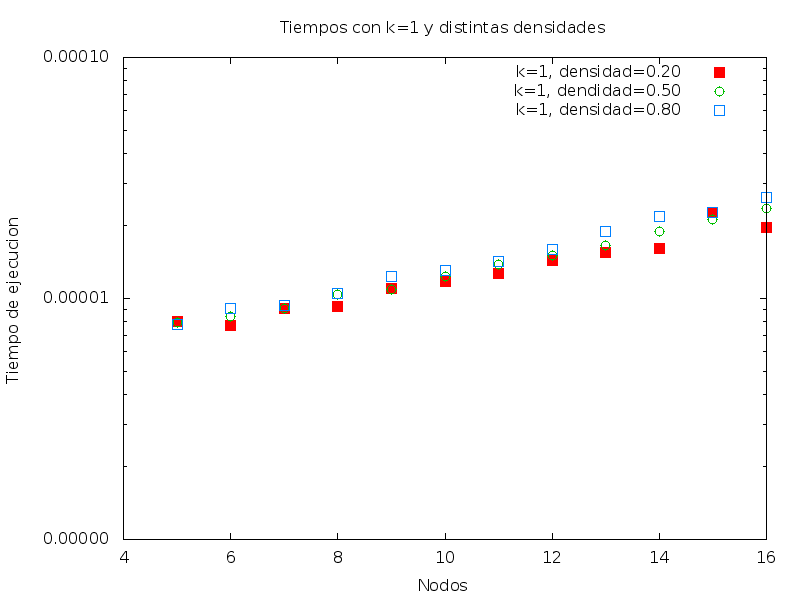
\includegraphics[scale=0.4]{ej2/k_1.png}
	\end{center}
	\caption{Comparaci\'on de k=1 con distintas densidades}
	\label{ej2_k_1}
\end{figure}

En el caso de $k=2$ \textbf{Figura \ref{ej2_k_2}}, podemos ver que el algoritmo se comporta mejor con grafos de densidad m\'as baja. Esto puede tener relaci\'on con el hecho de que al haber s\'olo dos posibilidades por v\'ertices y pocas aristas, es posible que en una rama lleguemos a una soluci\'on lo bastante buena como para podar muchas ramas.

\begin{figure}[H]
	\begin{center}
		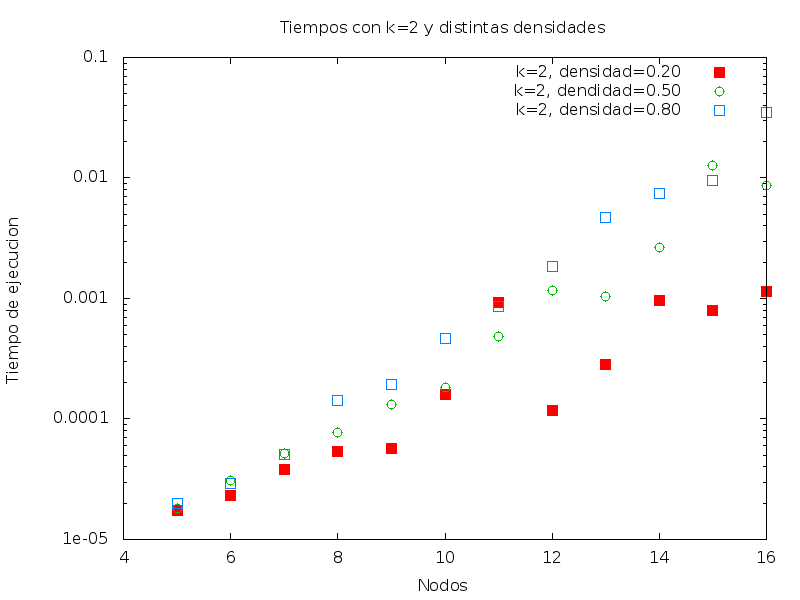
\includegraphics[scale=0.4]{ej2/k_2.png}
	\end{center}
	\caption{Comparaci\'on de k=2 con distintas densidades}
	\label{ej2_k_2}
\end{figure}

Si bien con $k=2$ parece que mejora con grafos poco densos, en la \textbf{Figura \ref{ej2_k_3}} y \textbf{\ref{ej2_k_4}} notamos como se va revirtiendo este comportamiento a medida que aumenta el k, hasta incluso, como se ve en la \textbf{Figura \ref{ej2_k_5}} parece que para 0.50 y 0.80 casi que obtenemos resultados similares.

\begin{figure}[H]
	\begin{center}
		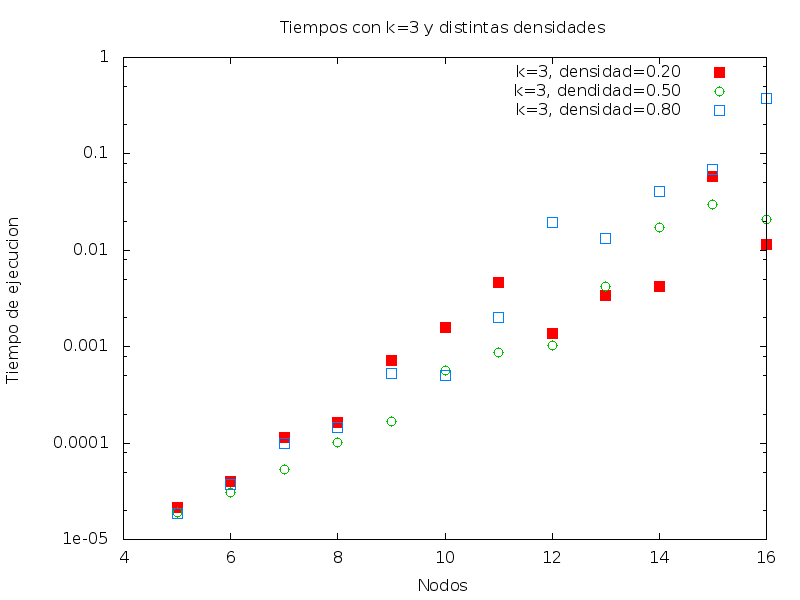
\includegraphics[scale=0.4]{ej2/k_3.png}
	\end{center}
	\caption{Comparaci\'on de k=3 con distintas densidades}
	\label{ej2_k_3}
\end{figure}

\begin{figure}[H]
	\begin{center}
		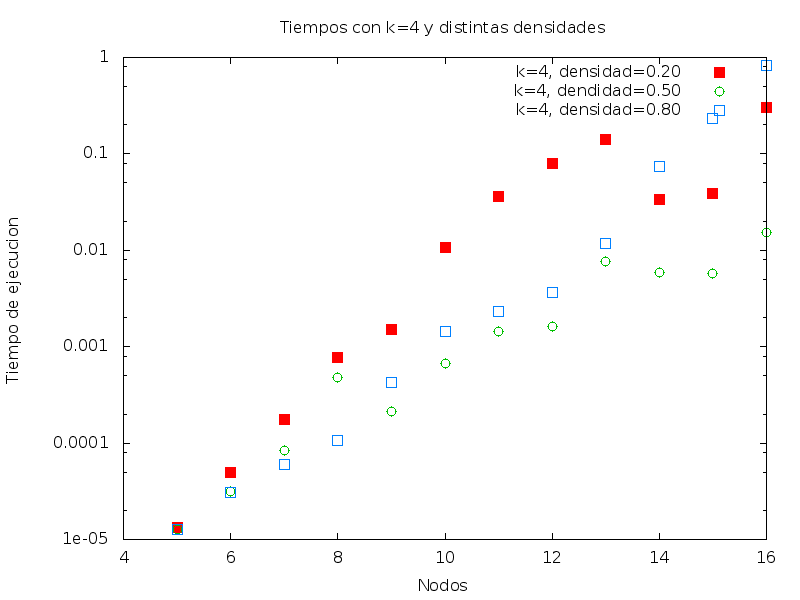
\includegraphics[scale=0.4]{ej2/k_4.png}
	\end{center}
	\caption{Comparaci\'on de k=4 con distintas densidades}
	\label{ej2_k_4}
\end{figure}

\begin{figure}[H]
	\begin{center}
		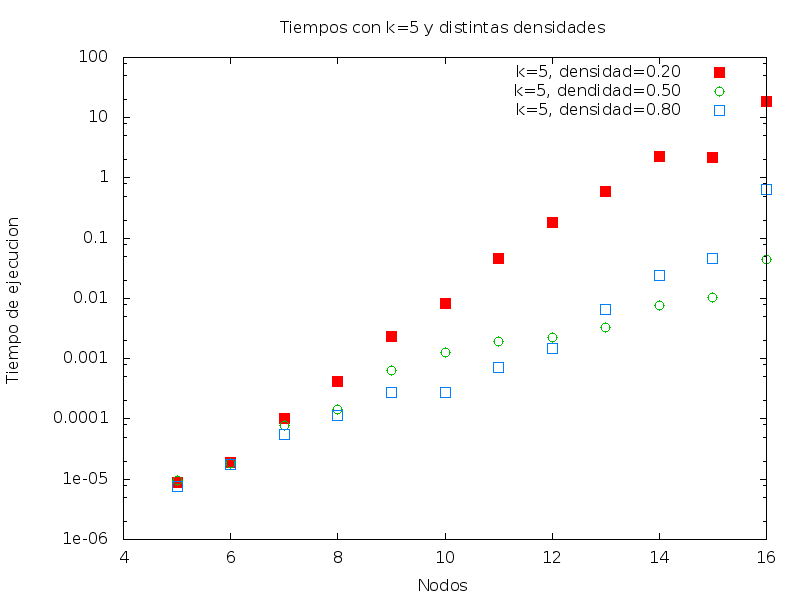
\includegraphics[scale=0.4]{ej2/k_5.png}
	\end{center}
	\caption{Comparaci\'on de k=5 con distintas densidades}
	\label{ej2_k_5}
\end{figure}

Estos resultados son anti intuitivos, pues uno creer\'ia que a menor densidad, mayor posibilidad de encontrar una soluci\'on buena y que con m\'as aristas mayor la necesidad de explorar el \'arbol. Esto puede estar sujeto al hecho de que a mayor cantidad de aristas, la probabilidad de cortar ramas aumenta, pues si la soluci\'on encontrada es de un peso considerablemente bajo, vamos a cortar en todas aquellas ramas que lo superen, esto siempre y cuando nos encontremos con un grafo con peso uniforme en las aristas y no con casos patol\'ogicos como aquel con todos pesos iguales, que nos obliga a recorrer el \'arbol entero.
\\
Otro factor interesante que modifica el comportamiento del algoritmo es cuan cerca est\'a $k$ de de $n$, por ejemplo, no siempre es cierto que el n\'umero de 5-Particiones de un conjunto es mayor que el n\'umero obtenido por un $k<5$ ya que si el conjunto tiene $6$ elementos, hay $15$ posibles 5-Particiones mientras que para $k=3$ hay $90$. Este n\'umero si bien no se mencion\'o con anterioridad corresponde el \textit{N\'umero de Stirling de Segunda Clase} y cada nivel del \'arbol de backtracking contiene la cantidad de k-particiones posibles para esa cantidad de nodos.
\\
Por \'ultimo, para mostrar que el algoritmo se comporta como lo indica la complejidad te\'orica, utilizamos k=5 y \'vertices del 5 al 16.

\begin{figure}[H]
	\begin{center}
		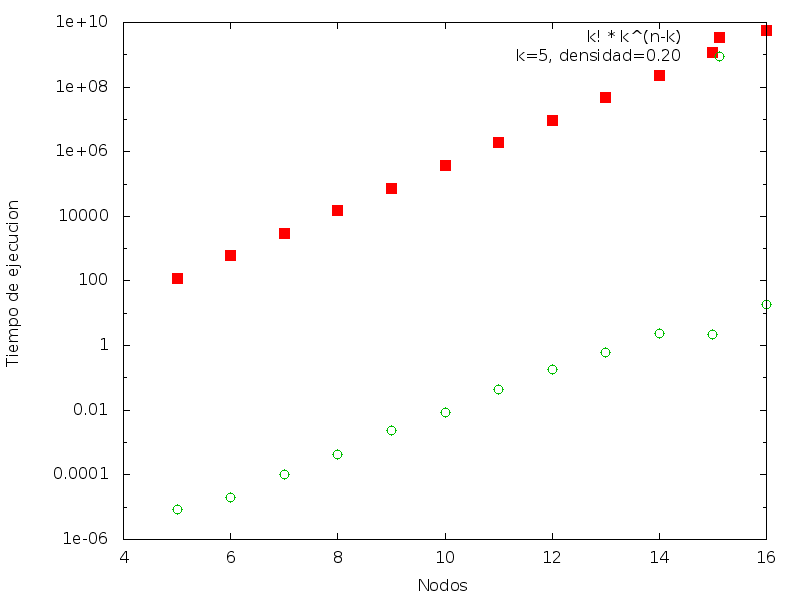
\includegraphics[scale=0.4]{ej2/teorico_k_5.png}
	\end{center}
	\caption{Comparaci\'on complejidad te\'orica contra las corridas sin poda para k=5}
	\label{ej2_teorico_k_5}
\end{figure}

Como se aprecia en la \textbf{Figura \ref{ej2_teorico_k_5}} el algoritmo se comporta de manera similar para un caso en que no le es posible aplicar la poda